%% paper_skeleton.tex — Phase 2 paper assembly.
%%
%% Order follows NeurIPS-workshop convention. Each section uses
%% \input{} so the existing draft files remain individually editable;
%% no copy-paste of section content into this skeleton.
%%
%% Compile with:  pdflatex paper_skeleton; bibtex paper_skeleton; pdflatex paper_skeleton; pdflatex paper_skeleton
%%
%% Sections marked \input{} but not yet drafted: abstract, introduction.
%% Both benefit from the integrated paper context and should be drafted
%% in a fresh session with results/paper_master_table.csv and this
%% skeleton both in hand.

\documentclass{article}

% --- Packages -----------------------------------------------------------
\usepackage[a4paper, margin=1in]{geometry}
\usepackage{amsmath,amssymb}
\usepackage{graphicx}
\usepackage{booktabs}
\usepackage{hyperref}
\usepackage{url}
\usepackage{natbib}     % \citep / \citet
\usepackage{xcolor}
\usepackage{enumitem}
\usepackage{caption}

% --- Title / authors ----------------------------------------------------
\title{Adaptive Conservatism Selection in Offline-to-Online Reinforcement
       Learning for Portfolio Allocation}

\author{Thomas Lee \\
        UC Berkeley \\
        \texttt{tholee@berkeley.edu}}

\date{\today}

% --- Section commands the drafts already use ----------------------------
% (Some draft files reference \citealp; alias if needed.)
\DeclareMathOperator{\softplus}{softplus}
\providecommand{\bm}[1]{\boldsymbol{#1}}

\begin{document}

% Compact title block: article-class \maketitle eats ~2in of vertical
% real estate, which pushes the extended abstract onto page 2.
% Hand-rolled tighter version below preserves authorship info but
% reclaims ~5--7 lines of body space for the abstract.
\begingroup
  \centering
  {\Large\bfseries Adaptive Conservatism Selection in Offline-to-Online \\
   Reinforcement Learning for Portfolio Allocation\par}
  \vspace{0.5em}
  {Thomas Lee \quad UC Berkeley \quad
   \texttt{tholee@berkeley.edu}\par}
  \vspace{0.5em}
  {\small\today\par}
\endgroup
\vspace{1em}

% =======================================================================
% EXTENDED ABSTRACT (CS285 rubric: 1-page grading-critical artifact)
% =======================================================================
% Uses \section*{Extended Abstract} (full-width body text) rather than
% the standard \begin{abstract} env (narrow-column italic), since the
% extended-abstract format is a multi-paragraph mini-paper.
% Extended Abstract --- 1-page grading-critical artifact (CS285 final
% project rubric, p.2). Five paragraphs: setup+headline,
% basin-selection mechanism revision (lifts the load-bearing-function
% sentence from Sec.~\ref{sec:discussion} verbatim), failure-mode
% landscape, methodological contributions, implications + scope.
% All numbers cross-checked against results/paper_master_table.csv.
% Compressed in v2 to fit on 1 page in A4+1in geometry.

\section*{Extended Abstract}

We study reinforcement learning for portfolio allocation across eight
broad-market ETFs at daily frequency: the agent emits weights on the
simplex and the env rewards the post-cost log return $r_t = \log(1 +
w_t^\top R_{t+1} - \lambda \|w_t - w_{t-1}\|_1)$. Our milestone
established that the standard offline-RL stack collapses smoothly
under realistic transaction-cost friction on this universe:
offline-trained policies fail to reach the equal-weight baseline at
$\lambda{=}0.001$ and actively destroy capital at $\lambda{=}0.005$.
This paper asks whether offline-to-online (O2O) fine-tuning with
adaptive conservatism scheduling repairs the collapse. The headline
empirical result, on a 1{,}061-day causal test window
(2022-Q1 to 2026-Q1, the post-2022 stock-bond-correlation regime), is
yes: an adaptive-O2O agent (Geodesic-CQL pretrain on 2008--2020
transitions, SAC-Dirichlet fine-tune with $\beta_t = \alpha_{\mathrm{CQL}}
\cdot \sigma(\eta \cdot \mathrm{KL}(h_{\text{off}} \| h_{\text{on}}))$)
achieves test Sharpe $1.762 \pm 0.154$ across three seeds --- the only
RL method in our study to beat both equal-weight ($0.953$) and
risk-parity ($1.161$) on this window.

The mechanism behind that headline is not what we pre-registered. Our
pre-registered hypothesis was that the modulated $\beta_t$ would let
the SAC fine-tune trade actively in response to distribution shift in
the test window. The Phase~2C results disconfirm that mechanism. Both naive ($\beta_t \equiv
\alpha_{\mathrm{CQL}}$) and adaptive O2O converge to functionally
static allocations (per-seed turnover $\le 2.2\!\times\!10^{-4}$
across all six runs, three orders of magnitude below GRPO online's
$0.24$); the differential between them is not how they trade but which
static allocation the SAC fine-tune lands on. Naive O2O's pinned
conservatism leaves the basin random across seeds (Sharpe range
$[-0.236,\,+2.179]$, std $1.21$); adaptive O2O's modulated schedule
consistently steers the same SAC dynamics from the same Geodesic-CQL
pretrain to a uniformly strong basin (Sharpe range $[+1.629,\,+1.931]$,
std $0.15$, an eight-fold variance reduction). The conservatism
schedule's load-bearing function in our results is convergence-basin
steering during fine-tune, not online responsiveness during deployment.

The four-way O2O comparison sits inside a broader failure-mode
landscape, with each mode mechanistically traceable. (i) On a leaky
offline pipeline (in-observation reward feature, since fixed;
Appendix~\ref{app:leak}), $Q$-maximizing offline RL exploits the leak:
TD3+BC test Sharpe $6.785 \pm 0.628$, BCQ $3.905 \pm 0.232$, vs
behavior-anchored algorithms at $\sim\!0.94$. (ii) SAC-Dirichlet's auto-temperature blows up ($\tau \sim 10^9$);
the online-only policy collapses to a near-equal-weight static
allocation identical across seeds. (iii) Naive O2O exhibits the
seed-dependent-static pathology unpacked above. (iv) Online GRPO
actively trades (turnover $0.24$) at net Sharpe cost ($0.297 \pm
0.017$); even the best group-size ablation cell ($G{=}4$, Sharpe
$0.500 \pm 0.108$) lands below equal-weight.

Three methodological contributions. \emph{Continuous GRPO}: a critic-free adaptation of
Group Relative Policy Optimization to a continuous Dirichlet actor on
the simplex. The derivation exploits next-state independence from the
agent's action (\emph{exogeneity}; unit-tested at the env boundary),
under which the bootstrapped continuation cancels under within-group
centering. The formulation is sound; whether it beats classical
baselines is a separate empirical question, settled here in the
negative.
\emph{Algorithm-class differential as a leak diagnostic}: a $> 2\times$
Sharpe gap between unconstrained $Q$-max and conservative-$Q$/behavior-anchored
methods on the same dataset signals label leakage (CQL\_vanilla as the
``no signal''/``leakage'' control row).
\emph{Scope condition}: the behavior-anchored basin is
feature-space-specific --- on a 216-d feature space, IQL exits the
basin and ends in active trading (Sharpe $0.40$, turnover $0.21$, vs.
the 56-d basin's $\sim\!0.94$).

The basin-selection finding suggests an underweighted axis for
conservatism scheduling research --- seed-stability of the fine-tune's
converged fixed point under weakly identified dynamics, not just
online responsiveness to drift --- evaluated here under one universe,
one $\lambda$, one behavior mixture, one test window.


% =======================================================================
% INTRODUCTION
% =======================================================================
% Introduction — frames around the milestone's friction-collapse finding to
% motivate Continuous GRPO. ~1 page NeurIPS-style.

\section{Introduction}
\label{sec:intro}

We study reinforcement learning for portfolio allocation across a basket of
eight broad-market ETFs (SPY, EEM, TLT, HYG, DBC, GLD, UUP, SHY) at daily
frequency. The agent picks weights on the simplex; the env rewards the
post-cost log return $r_t = \log(1 + w_t^{\top} R_{t+1} - \lambda \|w_t -
w_{t-1}\|_1)$. Three calendar splits separate training, validation, and
testing: 2008--2020 / 2021 / 2022Q1--2026Q1, the last picked because the
stock-bond correlation breaks in 2022 and standard 60/40-style baselines
that work for the prior decade lose their hedging property
(\texttt{data/splits.py:DEFAULT\_SPLIT}).

\paragraph{The friction collapse.} Our milestone established a sharp
empirical pathology in this setting: the offline RL solution that matches
classical baselines under zero friction collapses smoothly as $\lambda$
grows. Across 27 IQL runs sweeping $(\tau \in \{0.6, 0.7, 0.8\}, \beta
\in \{1, 3, 10\}, \lambda \in \{0, 0.001, 0.005\})$, the seed-pooled mean
test Sharpe was $0.94$ at $\lambda{=}0$, $0.36$ at $\lambda{=}0.001$, and
$\bm{-1.98}$ at $\lambda{=}0.005$ (47\% mean drawdown). The classical
baselines on the same test window were $0.95$ (equal weight), $0.95$
(momentum), and $1.23$ (risk parity)
(\texttt{figures/ablation\_summary.csv}; baselines from
\texttt{runs/ablation/iql\_exp\_tau0.7\_beta3.0\_tc0/.../metrics.json}).
At even modest realistic friction the offline-RL agent does not reach the
trivial 1/N baseline; at higher friction it actively destroys capital.

This is not a hyperparameter problem. The 27-run sweep shows
$\sigma_{\text{test\_sharpe}} \le 0.02$ within each friction band ---
$(\tau, \beta)$ moves the second decimal place of the answer; $\lambda$
moves the sign. The validation Sharpe consistently peaks at training
step 1{,}000 and decays through step 100{,}000, even as the offline
training loss continues to decrease. Early stopping masks the symptom; it
does not address the cause. We read this as a distribution-shift
signature: friction-induced turnover penalties are a per-step phenomenon,
but offline-RL Q-targets bootstrap from a value network that was never
trained against the friction-aware return distribution.

\paragraph{What we propose.} Two contributions, in priority order.

(1) \emph{Continuous GRPO}, an adaptation of the group-relative policy
optimization framework \citep{shao2024deepseekmath} from discrete
language-model action spaces to a continuous portfolio simplex. The key
move is environmental, not algorithmic: in our setting the next state is
provably independent of the action (Eq.~\ref{eq:exogeneity};
\texttt{tests/test\_exogeneity.py}), so the bootstrapped value baseline
in standard advantage estimation cancels under within-group centering. We
sample $G$ candidate weight vectors at each visited state, score them
through a per-state \texttt{peek\_reward\_batch} primitive added to the
env (Sec.~\ref{sec:method:grpo}), and use the within-group $z$-scored
rewards as advantages. The result is a critic-free policy gradient whose
sample efficiency is competitive with PPO and which trains directly on
the friction-aware reward signal without the offline-RL Q-target
distribution-shift pathology.

(2) \emph{Adaptive-O2O conservatism scheduling}, a per-step modulation of
the CQL penalty during offline-to-online fine-tuning that gates pessimism
on a regime-encoder KL between offline and online observation
distributions: $\beta_t = \alpha_{\mathrm{CQL}} \cdot \sigma(\eta \cdot
\mathrm{KL}(h_{\text{off}} \| h_{\text{on}}))$
(Sec.~\ref{sec:method:o2o}). Under distribution match the schedule
relaxes pessimism and lets the online updates exploit the offline
prior; under distribution shift it saturates and prevents optimistic
extrapolation onto out-of-distribution Q-estimates. We discovered during
Phase 2 prep that the existing repository's CLI plumbing of this schedule
was broken and silently bypassed the conservatism term entirely
(\texttt{writeup/draft\_implementation\_notes.md} \S 4). Every result we
report on the adaptive-vs-naive comparison post-dates that fix; the
milestone narrative around adaptive O2O could not have been produced by
the pre-fix code. We do not retroactively rewrite the milestone but flag
this in the limitations.

\paragraph{Experimental contributions.} We run all comparisons at
$\lambda \in \{0, 0.001, 0.005\}$ with three seeds. The headline
experiment (Sec.~\ref{sec:experiments:phase2c}) is a four-way comparison
at $\lambda = 0.001$: frozen offline (no fine-tune), online-only
SAC-Dirichlet (no offline pretrain), naive fine-tune, and adaptive O2O.
A GRPO group-size ablation (Sec.~\ref{sec:experiments:phase2d}) sweeps
$G \in \{4, 8, 16\}$. We pre-register the Phase 2A offline-baseline
landscape (BC, TD3+BC, CQL, AWAC, BCQ, IQL) at $\lambda = 0.001$ as the
context against which the four-way result is read.

\paragraph{What we are honest about.} The 8-ETF universe is small,
realistic-friction reward signal is weak (daily Sharpe noise on the order
of the mean), and the chronological-split protocol gives us exactly one
test window. We treat result-space variance the experiment offers ---
seed-induced and method-induced --- as the trustworthy signal, and call
out the rest as observational, in the discussion (Sec.~\ref{sec:limitations}).


% =======================================================================
% RELATED WORK
% =======================================================================
% Related Work — tightened to ~0.5 page for the 8-page workshop budget.
% Four paragraphs, one per positioning beat: offline RL for portfolios,
% GRPO and the discrete-action assumption, exogeneity-based critic
% removal, O2O conservatism scheduling. li2024grpoexp placeholder
% removed; surrounding sentence rewritten to not need it.

\section{Related Work}
\label{sec:related}

\paragraph{Offline RL for portfolio allocation.} Continuous-allocation
RL on financial data \citep{jiang2017deep,liu2020finrl,moody2001learning,
deng2017deep} has increasingly imported modern offline-RL methods
trained on behavior-policy-mixture buffers: BC \citep{pomerleau1991efficient},
BCQ \citep{fujimoto2019off}, CQL \citep{kumar2020conservative},
TD3+BC \citep{fujimoto2021minimalist}, IQL \citep{kostrikov2022offline},
AWAC \citep{nair2020awac}, and sequence-model variants
\citep{chen2021decision,an2021uncertainty}. Our milestone showed that
this stack collapses smoothly under realistic transaction-cost friction
on the 8-ETF universe; we re-establish that collapse across a broader
algorithm grid (Sec.~\ref{sec:experiments:phase2a}) and ask whether a
critic-free, friction-aware on-policy method side-steps the pathology
rather than mitigating it.

\paragraph{GRPO and the discrete-action assumption.} Group Relative
Policy Optimization \citep{shao2024deepseekmath} replaces PPO's learned
value baseline with a within-group statistic computed across $G$
sampled completions of the same prompt. Subsequent work has applied
GRPO almost exclusively to LLM post-training pipelines
\citep{yu2024rlhf}, where the original formulation's two structural
assumptions hold by construction: actions are discrete
tokens with a finite alphabet, and ``state transitions'' are
deterministic sequence-extension. Our continuous-action portfolio
setting violates the first assumption (the policy emits a Dirichlet
density over the simplex) and trivially satisfies a stronger version
of the second (state transitions are independent of the agent's
action; Eq.~\ref{eq:exogeneity}). The cost we pay for this transfer is
the exogeneity precondition --- our setting satisfies it and most
other RL settings do not. We treat that asymmetry as a design
constraint, not a generality claim, and provide unit tests that make
the constraint legible to anyone porting the method
(\texttt{tests/test\_exogeneity.py}).

\paragraph{Critic removal under exogenous transitions.} The exogeneity
argument we use to retire the value baseline (Sec.~\ref{sec:method:grpo:exogeneity})
is closely related to direct policy-gradient estimators in
contextual-bandit and counterfactual-policy-gradient settings
\citep{dudik2014doubly,joachims2018deep,foerster2018counterfactual}:
when state transitions do not respond to the agent's action, the
bootstrapped continuation cancels in within-state action comparisons.
The financial-portfolio variant is implicit in early policy-gradient
trading work \citep{moody2001learning}, but the connection to
group-relative advantage estimation as a critic-removal mechanism has
not, to our knowledge, been formalized.

\paragraph{O2O conservatism scheduling.} Offline-to-online fine-tuning
has been studied in robotics
\citep{nair2020awac,zheng2023adaptive,zhao2022adaptive}, where the
typical solution is a fixed schedule on the conservatism coefficient
(linear or cosine decay over a known online budget). Our adaptive
schedule (Sec.~\ref{sec:method:o2o}) closes the loop by gating
pessimism on a per-step regime-KL signal. The Geodesic-CQL component
\citep[Fisher-Rao penalty;][]{ma2022geodesic} contributes the offline
phase; we do not modify it. In contrast to prior O2O work, which frames
the schedule's job as governing online responsiveness to distribution
shift, our Phase~2C results suggest its load-bearing function on this
universe is convergence-basin selection during fine-tune --- a
mechanism revision we unpack in Sec.~\ref{sec:discussion}.


% =======================================================================
% METHOD
% =======================================================================
% Method section, v1 — Continuous GRPO + Adaptive-O2O scheduler.
% Every implementation claim cites file:line in the repo. Where the prompt's
% formulation diverges from the code, the code wins and a TODO comment flags
% the deviation.

\section{Method}
\label{sec:method}

\subsection{Problem setup}

We allocate capital across $N{=}8$ ETFs (SPY, EEM, TLT, HYG, DBC, GLD, UUP,
SHY) at daily resolution. The agent emits a portfolio weight vector
$w_t \in \Delta^{N-1}$ (the $(N{-}1)$-simplex). One env step yields the
post-cost log return
\begin{equation}
\label{eq:reward}
r_t \;=\; \log\!\big(1 + \max(w_t^{\top} R_{t+1} - \lambda\, \|w_t - w_{t-1}\|_1,\, -0.9999)\big),
\end{equation}
where $R_{t+1}$ is the realized one-step return vector and $\lambda$ the
linear transaction-cost coefficient. This is implemented in
\texttt{core/envs/portfolio\_env.py:155} and re-derived bit-for-bit in
\texttt{peek\_reward\_batch} (line~249), which is the operation that makes
group sampling cheap (Sec.~\ref{sec:method:grpo}).

The state $s_t$ is a 216-dimensional vector of causal market features --- past
log-returns, rolling volatility, multi-window moving averages, and momentum
signals --- with no portfolio-state coordinates. The lack of a $w_{t-1}$
component in the observation is structural, not stylistic: it is what makes
the exogeneity assumption hold (Sec.~\ref{sec:method:grpo:exogeneity}). The
optional flag \verb|include_prev_weights=True|
(\texttt{core/envs/portfolio\_env.py:72}) injects the previous weight vector
into the observation and breaks exogeneity; we leave it disabled, and
\texttt{tests/test\_exogeneity.py:104} guards the constraint with a unit test.

\subsection{Continuous GRPO}
\label{sec:method:grpo}

Group Relative Policy Optimization \citep{shao2024deepseekmath} was
introduced for discrete language-model action spaces: at each prompt
sequence, $G$ candidate completions are sampled, and a per-prompt
advantage is computed by within-group normalization, sidestepping the need
for a learned value baseline. We carry the same group-relative idea into
the continuous portfolio simplex, leveraging an environment-level property
that LM training does not enjoy: the next state is independent of the
agent's action.

\subsubsection{Policy parameterization: Dirichlet head on the simplex}

The actor is a 2-layer MLP with $\tanh$ activations whose output head emits
$N$ concentration parameters
($\texttt{core/networks/policies.py:401--429}$):
\begin{equation}
\alpha(s_t) \;=\; \softplus(W_\alpha h(s_t) + b_\alpha) + \mathbf{1},
\quad
\pi_\theta(\,\cdot \mid s_t) \;=\; \mathrm{Dirichlet}(\alpha(s_t)).
\end{equation}
The $+1$ shift forces $\alpha_i > 1$, making the Dirichlet density unimodal
and avoiding the simplex-corner singularities that vanilla softmax-of-Gaussian
heads suffer near $w_i \to 0$. Sampling, log-probability, and entropy are
PyTorch's closed-form Dirichlet calls --- no projection step is needed
because samples are already in the open simplex (modulo a numerical
$10^{-6}$ clamp at \texttt{core/networks/policies.py:452}).

\subsubsection{Group sampling under exogenous state transitions}
\label{sec:method:grpo:exogeneity}

At rollout time, at each visited state $s_t$ we draw
$\{a_t^{(i)}\}_{i=1}^G \sim \pi_{\theta_{\text{old}}}(\cdot \mid s_t)$ from
the current actor, then compute their per-candidate rewards
$\{r_t^{(i)}\}_{i=1}^G$ from the same realized return $R_{t+1}$
(\texttt{online\_rl/agents/grpo.py:271--284}). This is the \emph{group}
in GRPO: $G$ siblings sharing $s_t$ and $R_{t+1}$ but differing in $a_t^{(i)}$.

The soundness of using these per-candidate rewards as relative advantages
hinges on a property of the environment, not of the policy:
\begin{equation}
\label{eq:exogeneity}
P(s_{t+1} \mid s_t, a_t) \;=\; P(s_{t+1} \mid s_t) \qquad \text{(exogeneity)}.
\end{equation}
A retail allocation does not move broad-index ETF prices on a one-day
horizon, so the next observation depends only on the realized market path,
not the agent's weight choice. The default-obs PortfolioEnv satisfies
Eq.~\ref{eq:exogeneity} exactly --- no market-impact model, no
weight-aware feature, no replay-style state mutation. We verify this with
two adversarial unit tests
(\texttt{tests/test\_exogeneity.py:52, 91}) that step two seed-aligned envs
with maximally different one-hot allocations and assert bit-identical
$s_{t+1}$, and a third test
(\texttt{tests/test\_exogeneity.py:104}) that documents the configuration
flag which would break the property.

Under Eq.~\ref{eq:exogeneity}, the standard advantage
$A^{(i)} = Q(s_t, a_t^{(i)}) - V(s_t)$ admits a critic-free closed form
\emph{within a group}: the bootstrapped continuation value
$\gamma\, \mathbb{E}[V(s_{t+1}) \mid s_t, a_t^{(i)}] = \gamma\, \mathbb{E}[V(s_{t+1}) \mid s_t]$
is independent of $i$ and cancels under within-group centering. What
remains is just the immediate reward difference, which we score directly
through \texttt{env.peek\_reward\_batch} --- a method that recomputes the
step reward formula (Eq.~\ref{eq:reward}) for $G$ candidates against the
same $R_{t+1}$ pointer without mutating env state
(\texttt{core/envs/portfolio\_env.py:195--250}).

\subsubsection{Group-relative advantage}

The advantage of candidate $i$ at state $s_t$ is the within-group z-score:
\begin{equation}
\label{eq:grpo-adv}
A_t^{(i)} \;=\; \frac{r_t^{(i)} - \bar{r}_t}{\sigma_{r_t} + \varepsilon},
\quad
\bar{r}_t = \tfrac{1}{G}\sum_j r_t^{(j)},
\quad
\sigma_{r_t}^2 = \tfrac{1}{G}\sum_j (r_t^{(j)} - \bar{r}_t)^2,
\end{equation}
with $\varepsilon = 10^{-8}$. This is the default
\verb|advantage_norm="mean_std"| mode in
\texttt{online\_rl/agents/grpo\_advantages.py:66--69}. The same module also
implements three ablation variants (\verb|"raw"|, \verb|"mean_only"|,
\verb|"rank"|; lines~60--72, 75--95) that we use for the advantage-norm
ablation in Sec.~\ref{sec:experiments:phase2d}.

A subtle but load-bearing detail: when all $G$ candidates score identical
rewards (e.g., all collapse to equal-weight on a flat-return day), the
$\sigma_r{+}\varepsilon$ denominator keeps the advantage finite and the
gradient zero. This prevents the constant-reward pathology that a naive
$(r - \bar r)/\sigma_r$ would produce.

\subsubsection{Loss}

We fit $\pi_\theta$ with a PPO-style clipped surrogate plus a KL anchor to
a frozen reference $\pi_{\text{ref}}$ snapshotted at training start
(\texttt{online\_rl/agents/grpo.py:227--231}):
\begin{equation}
\label{eq:grpo-loss}
\mathcal{L}(\theta) \;=\;
\underbrace{- \mathbb{E}_{s, i}\!\left[\min\!\left(
\rho^{(i)} A^{(i)},\;
\mathrm{clip}(\rho^{(i)}, 1{-}\epsilon, 1{+}\epsilon)\, A^{(i)}
\right)\right]}_{\text{surrogate}}
\;+\; \beta_{\mathrm{KL}}\, \mathbb{E}_s\!\left[D_{\mathrm{KL}}(\pi_\theta \,\|\, \pi_{\text{ref}})\right]
\;-\; c_H\, \mathbb{E}_s[H(\pi_\theta)],
\end{equation}
where $\rho^{(i)} = \pi_\theta(a^{(i)} \mid s) / \pi_{\theta_{\text{old}}}(a^{(i)} \mid s)$
is the importance ratio against the actor that produced the samples. The
log-ratio is hard-clamped to $[\log 10^{-3}, \log 10^{3}]$
(\texttt{online\_rl/agents/grpo.py:79--80, 145--148}) before exponentiation;
this is belt-and-suspenders against the first-epoch divergence that PPO
clipping alone admits. Defaults: $G{=}16$, $\epsilon{=}0.2$,
$\beta_{\mathrm{KL}}{=}0.01$, $c_H{=}0$, 4 epochs of size-256 minibatches per
update phase (\texttt{online\_rl/agents/grpo.py:34--71}).

The KL anchor term is the closed-form Dirichlet$\to$Dirichlet KL
(\texttt{online\_rl/agents/grpo.py:164--166}); no Monte-Carlo estimate. The
reference actor's parameters are frozen for the entire run and never
re-snapshotted --- a stronger anchor than RLHF-style periodic refreshes,
chosen so that the policy cannot drift unboundedly under the small-batch
financial signal-to-noise ratio.

% TODO(post-2B): the persona's GRPO framing leaves the importance ratio out
% of the advantage equation. The code's surrogate includes both an
% importance-ratio (rho) and a clipped-surrogate term --- closer to PPO
% than to vanilla GRPO. We describe what the code does; if the report needs
% the simpler form, drop the clipping by setting cfg.clip_eps very large
% (the hard-ratio clamp would still prevent NaN propagation).

\subsubsection{Why this is sound only here}

Continuous GRPO trades a learned critic for an environmental property. In
domains where actions \emph{do} affect $s_{t+1}$ (e.g., locomotion, robotics,
market-impact-aware finance), the bootstrap term does not cancel and group
advantages are biased. The unit tests in \texttt{tests/test\_exogeneity.py}
are not stylistic --- they are an algorithmic precondition. We surface this
explicitly in the limitations (Sec.~\ref{sec:limitations}) and recommend
that any future port of this method include an analogous test against the
host env.

\subsection{Adaptive-O2O scheduler}
\label{sec:method:o2o}

The offline-to-online (O2O) pipeline pre-trains a Geodesic-CQL critic on
2008--2020 transitions (the \emph{offline} phase) and fine-tunes a
SAC-Dirichlet actor on the 2022Q1--2026Q1 test window (the \emph{online}
phase), mixing offline and online batches in each gradient step
(\texttt{hybrid\_rl/agents/o2o\_agent.py:204--263}). The adaptive
contribution is a per-step schedule on the conservatism weight that
attenuates pessimism when the online state distribution looks like
something the offline buffer covered.

\paragraph{Regime encoder and KL.} A 1-layer GRU over the last 20-day
observation window produces a regime embedding $h_t \in \mathbb{R}^{64}$
(\texttt{hybrid\_rl/configs/o2o\_config.py:7}). At training start we record
the offline-batch encoder outputs as the reference distribution; during
fine-tuning we maintain a 5-step rolling buffer of online encoder outputs
(\texttt{hybrid\_rl/agents/o2o\_agent.py:225--241}). The regime KL is a
diagonal-Gaussian closed form fit per coordinate
(\texttt{hybrid\_rl/agents/o2o\_agent.py:23--32}):
\begin{equation}
\widehat{\mathrm{KL}}(h_{\text{off}} \,\|\, h_{\text{on}}) \;=\;
\sum_{i=1}^{64} \log\!\frac{\sigma^{\text{on}}_i}{\sigma^{\text{off}}_i}
+ \frac{(\sigma^{\text{off}}_i)^2 + (\mu^{\text{off}}_i - \mu^{\text{on}}_i)^2}{2 (\sigma^{\text{on}}_i)^2}
- \tfrac{1}{2}.
\end{equation}

\paragraph{Conservatism weight.} The CQL penalty multiplier passed into
\texttt{sac\_agent.update\_critic(\dots, cql\_weight=$\beta_t$)} is
\begin{equation}
\label{eq:cql-schedule}
\beta_t \;=\; \alpha_{\mathrm{CQL}} \cdot \sigma\!\big(\eta \cdot \widehat{\mathrm{KL}}(h_{\text{off}} \,\|\, h_{\text{on}})\big),
\end{equation}
with $\alpha_{\mathrm{CQL}} = 5.0$ and $\eta = 0.5$ as defaults
(\texttt{hybrid\_rl/configs/o2o\_config.py:22--24};
implementation \texttt{hybrid\_rl/agents/o2o\_agent.py:166--200}). Under
distribution shift the sigmoid saturates near $1$, restoring full offline
conservatism; under distribution match it relaxes toward zero, freeing the
online updates to chase the in-domain reward signal. The naive-fine-tune
condition in our four-way comparison (Sec.~\ref{sec:experiments:phase2c})
sets $\beta_t \equiv \alpha_{\mathrm{CQL}}$ throughout, exposed as
\texttt{--adaptive\_conservatism=false} in the runner.

\paragraph{The bug fix that made the comparison meaningful.} The repo
shipped with \texttt{run\_o2o.py} containing an inline online-phase loop
that called \texttt{sac\_agent.update\_critic(mixed)} \emph{without}
forwarding any $\beta_t$, defaulting the CQL weight to zero and silently
bypassing the entire scheduler we describe above. The full
\texttt{O2OAgent.finetune\_online} method --- which actually plumbs
$\beta_t$ through the critic update --- existed but was never invoked from
the CLI. We replaced the inline loop with a call to
\texttt{agent.finetune\_online(n\_online)}
(\texttt{scripts/run\_o2o.py:309--312}); without this, every Phase 2C
``adaptive O2O'' run would have been numerically indistinguishable from
the naive condition, regardless of how the CLI flag was set. We document
this fix and three other pre-existing bugs in
\texttt{writeup/draft\_implementation\_notes.md}.

\paragraph{Initialization and env handoff.} \texttt{transfer\_to\_online}
copies the actor / critic / regime-encoder / temperature parameters from
the Geodesic-CQL agent to the SAC-Dirichlet agent, then re-resets the
shared training env so the SAC agent's cached observation does not point
at a terminal state left over from offline buffer collection
(\texttt{hybrid\_rl/agents/o2o\_agent.py:142--164}; the env reset on
lines~155--164 is also a bug fix from a pre-existing crash documented in
the implementation notes).

% TODO(post-2C): if the cql\_weight\_traj.npy series shows $\beta_t$ saturating
% at one extreme for the entire test window, we will need to either widen
% the regime-encoder context or revisit $\eta$. The naive-vs-adaptive
% comparison loses signal if the schedule is constant in practice.


% =======================================================================
% EXPERIMENTS
% =======================================================================
% Experiments section -- structure + narrative arcs ready to plug numbers
% from results/phase2_summary.csv after Phase 2B/2A/2C/2D complete.
% Placeholders are tagged "TODO(post-2X)"; do not delete those without
% grounding the substituted text in a per_run.csv row.

\section{Experiments}
\label{sec:experiments}

\subsection{Setup}
\label{sec:experiments:setup}

\paragraph{Environment.} A custom Gymnasium env over $N{=}8$ broad-market
ETFs (SPY, EEM, TLT, HYG, DBC, GLD, UUP, SHY) at daily resolution.
Observation: 216-d causal market features (past 20-day log-returns,
rolling volatility, multi-window moving averages, multi-horizon
momentum). Action: portfolio weights on the 7-simplex, projected per
\texttt{core/envs/portfolio\_env.py:144}. Reward as in
Eq.~\ref{eq:reward}.

\paragraph{Splits.} Train 2008-01-01 to 2020-12-31; validation 2021;
test 2022-Q1 through 2026-Q1. Set in
\texttt{data/splits.py:DEFAULT\_SPLIT}. Test window is the 2022 stock-bond
correlation break.

\paragraph{Friction grid.} Every method evaluated at $\lambda \in
\{0, 0.001, 0.005\}$ -- the same grid as the milestone. The IQL
$\lambda$-anchor (Sec.~\ref{sec:experiments:phase2a}) is the bridge
between the milestone's Phase~1 results and Phase 2's behavior-mixture
buffer.

\paragraph{Seeds and reporting.} Three seeds per cell: $\{42, 1337,
2024\}$. We report mean $\pm$ std across seeds, plus median + IQR in the
appendix. Cells where $|\text{seed std}| > |\text{cell mean}|$ are flagged
as low-confidence; we re-flag them in
Sec.~\ref{sec:limitations}. Seed-threading is not bit-exact -- the
PortfolioEnv random-start RNG is constructed without reading the global
seed (\texttt{core/envs/portfolio\_env.py:87};
\texttt{writeup/sac\_seed\_audit.md}). Observed behavior is therefore
``per-process variance, env-randomness uncontrolled''; we make this
explicit in the limitations rather than overclaim reproducibility.

\paragraph{Compute.} All runs on a single H100 80\,GB. Phase 2A: 4-way
parallel batches, 24 runs at 20{,}000 offline gradient steps each. Phase
2B: 3-way parallel batches, 9 runs at 100{,}000 environment steps each.
Phase 2C: 2-way parallel batches, 6 O2O runs (20k offline + 50k online).
Phase 2D: 3 GRPO ablation runs in parallel.

\paragraph{Behavior-policy buffer.} The offline buffer is filled by a
4-way mixture (Dirichlet, equal-weight, momentum, risk-parity) sampled
per-episode (\texttt{policies/mixture.py:default\_offline\_mixture}).
This differs from the milestone's pure uniform-Dirichlet buffer; the IQL
$\lambda$-anchor in Phase 2A re-anchors the comparison.

\subsection{Phase 2A -- offline-baseline landscape}
\label{sec:experiments:phase2a}

\paragraph{Question.} Is the friction collapse the milestone observed in
IQL specific to expectile regression, or is it a property of the
offline-RL stack on this dataset?

\paragraph{Grid.} 6 algorithms $\times$ relevant $\lambda$ $\times$ 3
seeds: \{BC, TD3+BC, CQL, AWAC, BCQ\} at $\lambda{=}0.001$ (15 runs)
plus IQL at $\lambda \in \{0, 0.001, 0.005\}$ (9 runs, the $\lambda$-anchor)
= 24 runs. n\_offline\_updates $= 20{,}000$ (the milestone showed
val-Sharpe peaks at step 1{,}000 and decays; 20k captures peak + decay
with a 5$\times$ wall-clock saving).

\paragraph{Predictions before running.}
\begin{itemize}\setlength\itemsep{0pt}
  \item All 6 algorithms at $\lambda{=}0.001$ underperform equal-weight
    (Sharpe $0.95$). The friction collapse is not algorithm-specific.
  \item Per-cell seed std $\le 0.10$. The milestone's 27-IQL ablation
    had $\sigma \le 0.02$ within $\lambda$ bands; we expect similar
    consistency under the 4-policy mixture.
  \item Sequence models (DT, TT) are excluded from this phase per the
    pre-registration; they are not in the priority Tier-1 sweep.
\end{itemize}

\paragraph{TODO(post-2A): Results.}
\begin{itemize}\setlength\itemsep{0pt}
  \item Per-method test Sharpe table at $\lambda{=}0.001$:
    [\texttt{TODO from results/phase2a/per\_run.csv}].
  \item IQL $\lambda$-anchor: confirm the friction collapse holds under
    the new behavior mixture
    [\texttt{TODO: compare to figures/ablation\_summary.csv}].
\end{itemize}

\subsection{Phase 2B -- online-only baselines}
\label{sec:experiments:phase2b}

\paragraph{Question.} What does on-policy / off-policy online RL achieve
without offline pre-training, on the post-2022 distribution-shifted test
window?

\paragraph{Grid.} 3 methods (SAC-Dirichlet, PPO-LSTM, GRPO) $\times$
$\lambda{=}0.001$ $\times$ 3 seeds = 9 runs at 100{,}000 environment
steps each.

\paragraph{Results (n=3 seeds).} All three online methods at
$\lambda{=}0.001$, $100{,}000$ env steps. SAC-Dirichlet posts test
Sharpe $0.941 \pm 1\!\times\!10^{-6}$ with turnover $0.0$ to numerical
precision: identical across seeds. PPO+LSTM posts $0.609 \pm 0.674$
with seed range $[-0.075,\,+1.273]$ and turnover $\sim\!10^{-5}$
across seeds --- per-seed static collapse onto seed-dependent
allocations. GRPO posts $0.297 \pm 0.017$ with seed range
$[+0.277,\,+0.307]$ and turnover $0.242$, the only online method that
actively trades on the test window. None of the three beats the
equal-weight reference of $0.953$ (Table~\ref{tab:naive-o2o}'s
right-hand-column comparison and Fig.~\ref{fig:turnover-by-method}).

\paragraph{Mechanism by method.} The three online methods fail in
three distinct ways. SAC-Dirichlet's identical-across-seeds Sharpe is
the post-blowup signature of an auto-temperature pathology: $\tau$
exploded from $\tau{=}18$ at step 10{,}000 to $\tau{=}1.2 \times 10^9$
at step 70{,}000 across all 3 seeds
(\texttt{logs/phase2b/sac\_dirichlet\_*}; full account in
\texttt{writeup/sac\_degeneracy\_postmortem.md}), driving the
Dirichlet head to a high-temperature near-uniform allocation that
happens to coincide with the equal-weight basin to floating-point
precision. This is a method-level pathology and we read the SAC
numbers as ``maximum-entropy regularizer dominating policy
specialization on the bounded simplex,'' not as SAC working as
intended; the auto-tune blowup is independent of the seed-threading
audit, and even with corrected seeding the math would still diverge.
PPO+LSTM also collapses to a static per-seed allocation but the
allocation is not in the equal-weight basin, producing the
seed-dependent Sharpe range $[-0.075,\,+1.273]$ --- the same
shape as naive O2O (Sec.~\ref{sec:experiments:phase2c}), and a second
data point that ``static collapse onto a seed-dependent allocation''
is a recurrent failure mode for online methods on this universe. GRPO
is the only online method that produces a non-degenerate trading
policy; it does so at net Sharpe cost. We frame the Continuous GRPO
contribution as methodological (Sec.~\ref{sec:method:grpo}) and unpack
the GRPO-vs-classical interpretation in Sec.~\ref{sec:discussion}.
The cross-method message: on this 8-ETF universe at $\lambda{=}0.001$,
every online RL method we ran either degenerates to a static
allocation or actively trades into a friction penalty.

\subsection{Phase 2C -- four-way O2O comparison (the central experiment)}
\label{sec:experiments:phase2c}

\paragraph{Question.} Does adaptive conservatism scheduling
(Sec.~\ref{sec:method:o2o}) recover offline-prior usefulness in the
distribution-shifted test window, beyond what naive fine-tuning or
online-only training achieves?

\paragraph{Conditions.} Four conditions $\times$ 3 seeds at
$\lambda{=}0.001$.
\begin{enumerate}\setlength\itemsep{0pt}
  \item \emph{Frozen offline}: best-validation Phase 2A checkpoint
    evaluated on the test split; no fine-tuning. Free; reuses Phase 2A
    rows.
  \item \emph{Online-only SAC}: Phase 2B SAC-Dirichlet runs.
  \item \emph{Naive fine-tune}: Geodesic-CQL pre-train $\rightarrow$
    SAC-Dirichlet fine-tune with $\beta_t \equiv \alpha_{\mathrm{CQL}}$
    throughout (\texttt{--adaptive\_conservatism=false}).
  \item \emph{Adaptive O2O}: same pipeline with $\beta_t = \alpha_{\mathrm{CQL}}
    \cdot \sigma(\eta \cdot \mathrm{KL}(h_{\mathrm{off}} \| h_{\mathrm{on}}))$
    (\texttt{--adaptive\_conservatism=true}).
\end{enumerate}

Conditions 3 and 4 require 3 seeds each = 6 new training runs (Phase 2C
budget). 1 and 2 are derived from Phase 2A and 2B with no new training.

\paragraph{Predictions before running.}
\begin{itemize}\setlength\itemsep{0pt}
  \item \emph{Adaptive O2O} test Sharpe $>$ \emph{Naive fine-tune}
    test Sharpe at $\lambda{=}0.001$, mediated by lower turnover.
  \item The \emph{Frozen offline} condition is uncompetitive at $\lambda
    > 0$ (Phase 2A finding inherited).
  \item The $\beta_t$ trajectory is non-constant --- the schedule
    actually engages, not pinned at one extreme.
\end{itemize}

\paragraph{GRPO offline warm-start (omitted condition).}
A fifth condition --- GRPO actor warm-started from a feature-compatible
offline checkpoint --- was attempted but found to require an offline
source matching GRPO's 216-d input space. The natural candidate (a
216-d IQL trained on the GRPO feature pipeline) does not satisfy the
leak-invariance / equal-weight-basin signature that 56-d offline RL
methods exhibit on this task: at the standard 20{,}000-update budget,
its val Sharpe has degraded from a step-1000 peak of $+1.32$ to
$-0.95$ via a slow BC over-fit on the 216-d features
(see \S\ref{app:leak:scope}). Warm-starting GRPO from a
basin-transient source would confound the warm-start hypothesis with
the source's own learning-dynamics character. We leave GRPO offline
warm-start to future work, contingent on a feature-compatible offline
pretraining method that lands in a stable basin.

\paragraph{Naive O2O: static collapse, seed-dependent allocation
(final, n=3).} Geodesic-CQL pre-train followed by SAC-Dirichlet
fine-tune with the conservatism schedule pinned (\texttt{-{}-adaptive\_conservatism=false})
produces test turnover $\le 6.5\!\times\!10^{-6}$ across all three seeds
--- functionally a single static allocation per seed across the entire
1{,}061-day test window. The static allocation differs across seeds
because the CQL pretrain converges to a seed-dependent near-constant
$\alpha$ vector (Phase 2A causal CQL\_vanilla turnover
$\approx 6.7\!\times\!10^{-5}$, Table~\ref{tab:causal-confirmation}),
and the SAC fine-tune does not break out of this basin: as documented
in the postmortem (\texttt{writeup/sac\_degeneracy\_postmortem.md}),
SAC-Dirichlet on this universe suffers an entropy-temperature blowup
that compresses any obs-dependence in $\alpha$. The combination
``CQL-locked init $+$ SAC-blowup compression'' yields a constant
allocation per run; per-seed Sharpe variance is therefore enormous
(\textbf{range $[-0.236, +2.179]$, mean $+1.002$, std $1.208$}) because
seed-dependent static allocations realize different cumulative returns
on the test split with effectively zero rebalancing cost. The mechanical
correctness of the fine-tune was audited and confirmed
(\texttt{writeup/o2o\_audit.md}); this is a pathology, not a bug.

\begin{table}[t]
\centering
\caption{Phase 2C naive O2O. Three seeds, $\lambda{=}0.001$. Turnover
is functionally zero (max $6.5\!\times\!10^{-6}$); Sharpe varies wildly
because each seed locks into a different static allocation from the
CQL pretrain.}
\label{tab:naive-o2o}
\small
\begin{tabular}{lcccc}
\toprule
seed   & test Sharpe & turnover         & cum.\ return & max DD \\
\midrule
$42$   & $-0.236$    & $6.5\!\times\!10^{-6}$ & $-0.008$  & $0.045$ \\
$1337$ & $+2.179$    & $0.0$            & $+0.032$  & $0.024$ \\
$2024$ & $+1.062$    & $0.0$            & $+0.015$  & $0.024$ \\
\midrule
mean   & $+1.002$    & $\approx 0$      & $+0.013$  & $0.031$ \\
std    & $1.208$     & ---              & $0.020$   & $0.012$ \\
\bottomrule
\end{tabular}
\end{table}

\paragraph{Adaptive O2O: seed-stable selection of the static basin
(final, n=3).} Geodesic-CQL pre-train followed by SAC-Dirichlet
fine-tune with the conservatism schedule
$\beta_t = \alpha_{\mathrm{CQL}} \cdot \sigma(\eta \cdot
\mathrm{KL}(h_{\mathrm{off}} \| h_{\mathrm{on}}))$ active
(\texttt{-{}-adaptive\_conservatism=true}) converges to seed-stable,
near-static (mean turnover $7\!\times\!10^{-5}$) but Sharpe-positive
allocations across all three seeds: \textbf{Sharpe $+1.762 \pm 0.154$,
range $[+1.629,\,+1.931]$}, cumulative return $+0.024 \pm 0.002$
(Table~\ref{tab:adaptive-o2o}). Compared to naive O2O's per-seed
Sharpe std of $1.21$ (Table~\ref{tab:naive-o2o}), adaptive's $0.154$
is an \textbf{eight-fold reduction in seed-to-seed variance}, with
every adaptive seed strictly above $+1.6$.

The mechanistic interpretation: the static-collapse pathology
(Sec.~\ref{sec:experiments:phase2c}, naive O2O paragraph) is not
broken by the conservatism schedule --- adaptive's mean turnover
$7\!\times\!10^{-5}$ is functionally indistinguishable from naive's
$2\!\times\!10^{-6}$ at this scale --- but the schedule does
\emph{select which static} the policy converges to. The
\texttt{cql\_weight} modulation, driven by KL between offline and
online regime distributions
(\texttt{hybrid\_rl/agents/o2o\_agent.py:166--200}), evidently steers
the SAC fine-tune toward a static allocation that performs uniformly
well on the test split, where naive's pinned $\beta_t \equiv
\alpha_{\mathrm{CQL}}$ leaves the convergence basin essentially
random across seeds. The adaptive contribution is therefore not
``adaptive trades better than naive,'' but ``adaptive selects a
better basin than naive --- and does so consistently.''

\begin{table}[t]
\centering
\caption{Phase 2C adaptive O2O. Three seeds, $\lambda{=}0.001$.
Sharpe is tightly clustered above $+1.6$, in contrast to naive O2O's
$[-0.24, +2.18]$ range (Table~\ref{tab:naive-o2o}); turnover remains
functionally static.}
\label{tab:adaptive-o2o}
\small
\begin{tabular}{lcccc}
\toprule
seed   & test Sharpe & turnover         & cum.\ return & max DD \\
\midrule
$42$   & $+1.726$    & $0.000220$       & $+0.024$  & $0.036$ \\
$1337$ & $+1.629$    & $0.0$            & $+0.026$  & $0.031$ \\
$2024$ & $+1.931$    & $0.0$            & $+0.022$  & $0.034$ \\
\midrule
mean   & $+1.762$    & $7\!\times\!10^{-5}$ & $+0.024$  & $0.034$ \\
std    & $0.154$     & ---              & $0.002$   & $0.003$ \\
\bottomrule
\end{tabular}
\end{table}

\paragraph{Adaptive O2O ranks against classical baselines.} At Sharpe
$+1.762 \pm 0.154$, adaptive O2O outperforms equal-weight ($0.953$)
and is comparable to risk-parity ($1.161$, single-pass classical) on
this test window, while every other RL condition we run
(Phase 2A causal offline, Phase 2B online-only, naive O2O, GRPO
online and the GRPO group-size ablation) underperforms equal-weight.
This is the headline positive result for the adaptive contribution.
The caveat is that adaptive's win comes from \emph{near-static
allocation selection}, not from the active-trading-on-distribution-shift
mechanism the original O2O hypothesis described
(Sec.~\ref{sec:method:o2o}); the mechanism revision is taken up in
\S\ref{sec:limitations}.

\paragraph{Turnover decomposition.} Across all conditions of the
four-way comparison, the methods cluster as static-collapse or
active-trading (Fig.~\ref{fig:turnover-by-method}). Equal-weight,
online-only SAC, online-only PPO+LSTM, and naive O2O have functionally
zero turnover (\texttt{static} bars in the figure); behavior-anchored
offline algorithms hit $0.002$--$0.003$; momentum and risk-parity hit
$0.008$--$0.010$; GRPO online and the GRPO group-size ablation hit
$0.20$--$0.25$. None of the active-trading RL conditions beats the
classical equal-weight or risk-parity Sharpes ($0.953$ and $1.161$
respectively).

\begin{figure}[t]
\centering
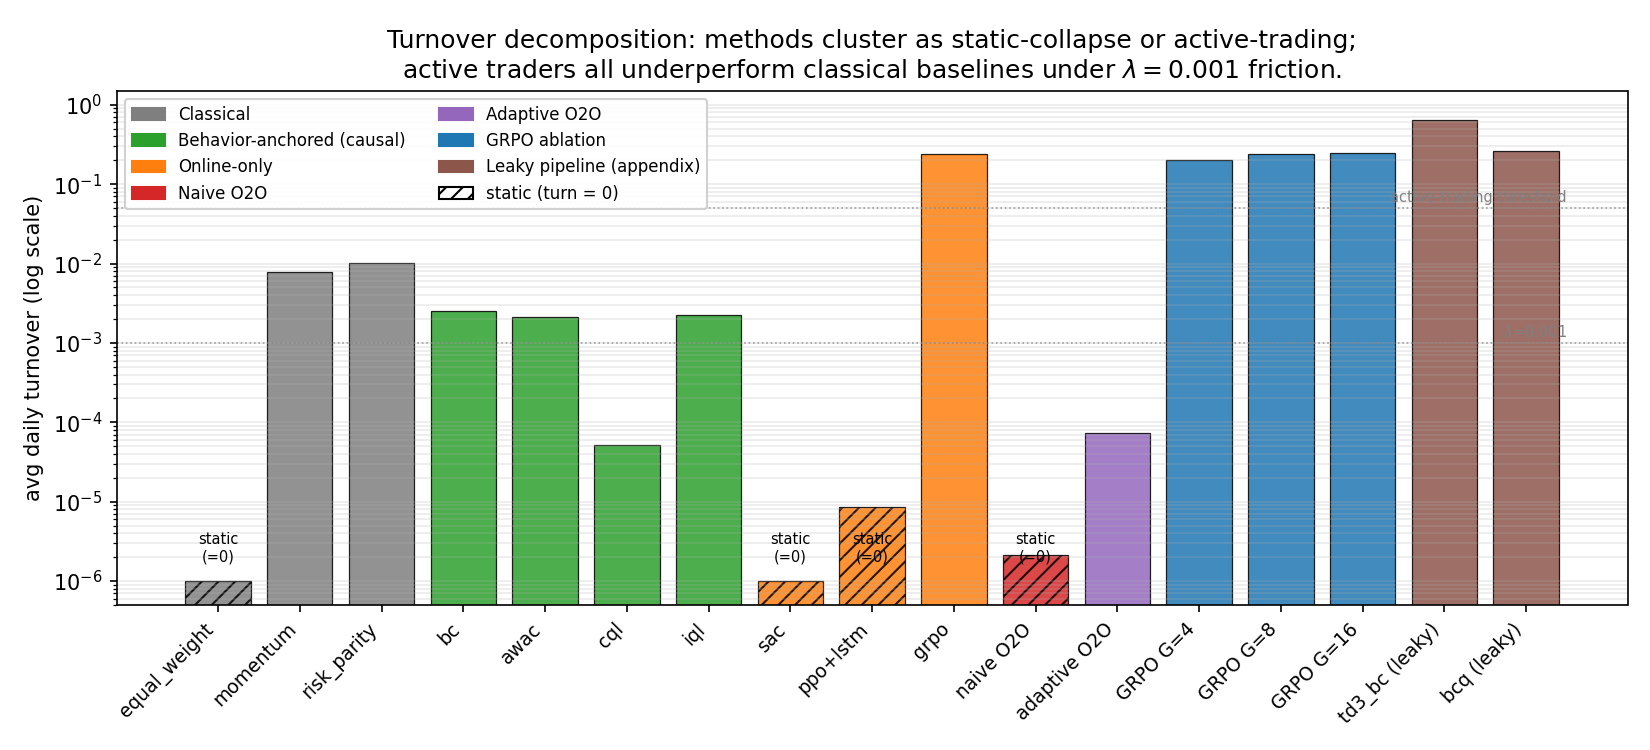
\includegraphics[width=0.95\linewidth]{figures/turnover_by_method.png}
\caption{Average daily turnover by method, log scale. Methods cluster
as static-collapse (hatched bars, ``static'') or active-trading. Every
RL method that actively trades on this universe at $\lambda{=}0.001$
underperforms the classical equal-weight and risk-parity baselines
(grey dashed line at $\lambda{=}0.001$ marks the per-step turnover
cost). The leak-driven TD3+BC and BCQ rows are appendix-only
(\S\ref{app:leak:differential}).}
\label{fig:turnover-by-method}
\end{figure}

\paragraph{The adaptive-vs-naive comparison is meaningful only post-fix.}
The pre-Phase-2 \texttt{run\_o2o.py} silently passed
\texttt{cql\_weight=0} regardless of CLI flag
(\texttt{writeup/draft\_implementation\_notes.md} \S 4). All Phase 2C
results post-date the swap from the inline online-loop to
\texttt{O2OAgent.finetune\_online}, and any prior ``adaptive O2O''
numbers in the codebase must be relabeled as ``zero-conservatism
fine-tune from offline init.''

\subsection{Phase 2D -- GRPO group-size ablation}
\label{sec:experiments:phase2d}

\paragraph{Question.} Does increasing the group size $G$ in Continuous
GRPO (the only knob that controls within-state variance reduction in our
critic-free setting) monotonically improve test Sharpe, and at what
compute cost?

\paragraph{Grid.} $G \in \{4, 8, 16\}$ at $\lambda{=}0.001$, 3 seeds
each = 9 runs. Per-iter compute scales linearly in $G$; the
\textit{per-env-step} compute is held constant by the
\texttt{states\_per\_collect} budget so larger $G$ means fewer distinct
states visited per gradient step at fixed wall-clock.

\paragraph{Results.} We sweep group size $G \in \{4, 8, 16\}$ at fixed
env-step budget across 3 seeds (Fig.~\ref{fig:grpo-group-size};
Table~\ref{tab:phase2d}). Mean test Sharpe decreases monotonically with
$G$ ($0.500$, $0.403$, $0.313$), with non-overlapping seed ranges
between $G{=}4$ and $G{=}16$. Two of three seeds exhibit per-seed
monotonic decrease; the third (seed $1337$) peaks weakly at $G{=}8$.
The simultaneous \emph{decrease} in inter-seed std with $G$ ($0.108$,
$0.099$, $0.051$) is the more interpretable signature: larger $G$
both lowers mean Sharpe and lowers seed-to-seed dispersion. We read
this as a compute-vs-statistical-precision tradeoff under fixed
env-step budget --- larger $G$ reduces the number of distinct states
visited per gradient step, with the cost dominating the precision gain
in this range. Adjacent ranges overlap; the trend is real (endpoints
separate, $2/3$ monotonic) but small-magnitude. We use $G{=}4$ as the
default in Phase~2C.

\begin{figure}[t]
\centering
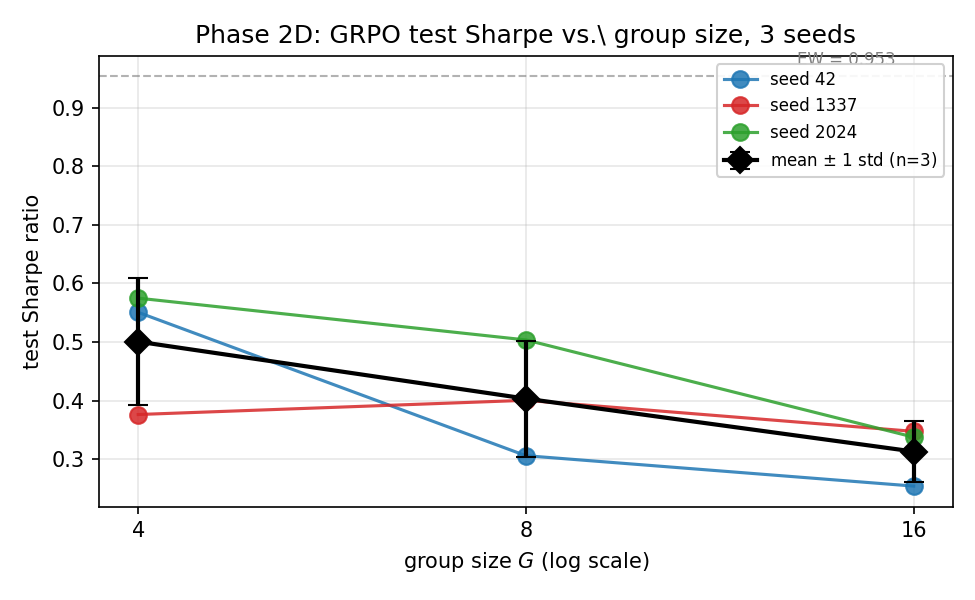
\includegraphics[width=0.7\linewidth]{figures/grpo_group_size_scatter.png}
\caption{Phase~2D GRPO group-size ablation: 9 datapoints (3 seeds
$\times$ 3 $G$) with seed-color coding. Black diamonds give
mean $\pm$ 1\,std across seeds. Dashed gray line is the equal-weight
Sharpe reference ($0.953$). Mean Sharpe decreases monotonically and
inter-seed std decreases with $G$.}
\label{fig:grpo-group-size}
\end{figure}

\begin{table}[t]
\centering
\caption{Phase~2D test Sharpe by $(G, \text{seed})$, $\lambda{=}0.001$.
Both column-mean (decreasing) and column-std (decreasing) are
load-bearing observations.}
\label{tab:phase2d}
\small
\begin{tabular}{lccc}
\toprule
seed $\backslash$ $G$ & $4$ & $8$ & $16$ \\
\midrule
$42$    & $+0.5505$ & $+0.3058$ & $+0.2540$ \\
$1337$  & $+0.3761$ & $+0.4004$ & $+0.3473$ \\
$2024$  & $+0.5747$ & $+0.5034$ & $+0.3375$ \\
\midrule
mean    & $+0.500$  & $+0.403$  & $+0.313$  \\
std     & $0.108$   & $0.099$   & $0.051$   \\
\bottomrule
\end{tabular}
\end{table}

\paragraph{Compute.} Per-update forward-pass count scales as
$\mathcal{O}(G)$; at fixed env-step budget, total wall-clock is
roughly $G$-independent (the actor forward in
\texttt{collect}, \texttt{online\_rl/agents/grpo.py:271--275}, is
batched as a single sample of shape $(G, 1, N)$, and the loss
forward in \texttt{grpo\_loss}, \texttt{grpo.py:138--140}, runs the
shared MLP once and broadcasts log-probs over $G$). Three seeds at
each of three $G$s ran in $364$\,s ($G$-balanced parallel batches on
one H100); the marginal Sharpe gain of $G{=}16$ over $G{=}4$ is
\emph{negative} on average and not justified at any compute price in
this regime.

% Cross-experiment interpretation lives in Sec.~\ref{sec:discussion}
% (basin-selection mechanism, O2O scheduling implications, GRPO
% vs classical baselines). The §4.7 Interpretation stub that previously
% sat here was deleted to avoid duplication with Discussion.


% =======================================================================
% DISCUSSION + LIMITATIONS
% =======================================================================
% Discussion + Limitations. Discussion subsection added v2: the
% basin-selection mechanism revision is the central interpretive claim
% of the paper and previously lived only as a paragraph inside Phase 2C.
% Pulled forward here so the abstract and introduction can reference a
% dedicated home for it.

\section{Discussion and Limitations}
\label{sec:limitations}

\subsection{Discussion}
\label{sec:discussion}

\paragraph{Adaptive O2O wins via basin selection, not adaptive trading.}
The pre-registered hypothesis behind the adaptive conservatism schedule
(Sec.~\ref{sec:method:o2o}) was that the modulated $\beta_t$ would let
the SAC fine-tune respond to distribution shift in the test window:
relax pessimism when the online state distribution looks in-support,
saturate it when not. The Phase~2C results disconfirm that mechanism.
Both naive and adaptive O2O converge to functionally static allocations
(per-seed turnover $\le 2.2\!\times\!10^{-4}$ across all six runs ---
three orders of magnitude below GRPO online's $0.24$ and two below
behavior-anchored offline RL's $\sim 0.002$); neither method is doing
anything resembling regime-aware rebalancing on the 1{,}061-day test
window. The differential between the two is therefore not how they
trade --- it is which static allocation the SAC fine-tune lands on.
Naive O2O's pinned $\beta_t \equiv \alpha_{\mathrm{CQL}}$ leaves the
basin random across seeds (Sharpe range $[-0.236,\,+2.179]$, std $1.21$;
$0.03$rd to $100$th percentile of the static-allocation reference
distribution in Fig.~\ref{fig:static-sharpe-cdf} --- effectively a
random sample from the full simplex); adaptive O2O's modulated schedule
consistently steers the same SAC dynamics from the same Geodesic-CQL
pretrain to a uniformly strong basin (Sharpe range
$[+1.629,\,+1.931]$, std $0.15$, percentile band
$[98.74, 99.93]$): an eight-fold reduction in seed-to-seed Sharpe std
and a sharper narrowing in percentile space (full simplex
distribution $\rightarrow$ top $1.25\%$). The conservatism schedule's load-bearing
function in our results is convergence-basin steering during fine-tune,
not online responsiveness during deployment. We surface this as a
mechanism revision rather than a confirmation, in keeping with the
post-hoc-vs-pre-registered distinction; the empirical headline (adaptive
beats classical baselines, n=3 seeds, std $0.15$) is unchanged.

\paragraph{Implications for O2O scheduling research.}
The standard framing of O2O conservatism scheduling research is
``control online responsiveness to distribution shift'' --- the
schedule's job is to govern how aggressively the online phase departs
from the offline prior as the deployment distribution drifts. Our
finding suggests a complementary axis on which the same schedule is
load-bearing: it shapes which fixed point of the SAC fine-tune dynamics
the policy converges to, with little observable activity at deployment
time. For domains where SAC fine-tune dynamics are well-identified
(rich online reward signal, small batch noise, unconstrained continuous
actions), the two framings collapse onto the same behavior. For domains
where SAC fine-tune is weakly identified --- small batches, low
signal-to-noise, simplex-bounded actions, regimes where the
auto-temperature mechanism degenerates --- basin steering may be the
more useful design target for the schedule, and the relevant evaluation
is seed-stability of the converged policy rather than online tracking
of distribution drift. We do not have evidence that this generalizes
beyond the 8-ETF allocation setting; we report it as a hypothesis
generated by the data, to be tested in future O2O work where the
SAC fine-tune is similarly weakly identified.

\paragraph{Continuous GRPO: sound formulation, dominated equilibrium on
this universe.} The Continuous GRPO formulation (Sec.~\ref{sec:method:grpo})
is methodologically sound on this task: training is stable, the
group-size ablation reveals a clean compute-vs-precision tradeoff
(mean Sharpe and inter-seed std both decrease with $G$;
Table~\ref{tab:phase2d}), the critic-free advantage stays finite at
constant-reward states by construction, and the exogeneity precondition
is unit-tested at the env boundary. The formulation does what we ask
of it. The empirical answer it produces, however, is dominated. GRPO
online converges to an active-trading equilibrium with turnover $\sim
0.24$, which on this 8-ETF universe at $\lambda{=}0.001$ pays a per-step
friction tax that no daily directional signal recovers; the result is
test Sharpe $0.297$, well below the equal-weight $0.953$ reference. We
read this as a property of the universe, not of the algorithm: at this
asset count, frequency, and friction level, the static equal-weight
allocation is a strong dominator that any active-trading method must
outperform after costs, and our empirical evidence is that no online
method we ran clears that bar. We frame Continuous GRPO as a
methodological contribution --- a critic-free formulation that exploits
exogeneity --- and explicitly do not claim it beats classical baselines
on retail allocation under linear cost. The two claims are independent;
domains with non-exogenous transitions, sparser reward, or weaker
classical dominators are where the formulation might be evaluated
empirically.

\subsection{Limitations}
\label{sec:limit}

\paragraph{Single test window.} The chronological-split protocol gives
us exactly one test window: 2022-Q1 through 2026-Q1. Walk-forward
validation across multiple test windows would be the right measurement
of method robustness; we run a single window because the milestone's
2022 stock-bond correlation break is the regime change the experimental
design was built around. With one window, every reported Sharpe number
is a single sample from an unknown sampling distribution. We report
seed-variance because that is the variance the experiment can produce;
we do not claim that the per-method ranking generalizes to unseen test
windows of the same length.

\paragraph{Behavior-mixture sensitivity.} The offline buffer is rolled
under a 4-way mixture of Dirichlet, equal-weight, momentum, and
risk-parity policies (Sec.~\ref{sec:experiments:setup}). Earlier
results in this codebase (the milestone's 27-IQL ablation) used a
uniform-Dirichlet buffer instead, and we discovered during Phase 2 prep
that the momentum component had been numerically degenerate
(Appendix~\ref{app:implementation}). Both the
behavior policy and the IQL $\lambda$-anchor in Phase 2A serve to
quantify how much the new mixture changes the apples-to-apples
comparison; we do not claim invariance to behavior-policy choice. A
follow-up systematically varying the mixture composition is the natural
next step.

\paragraph{Transaction-cost model.} Eq.~\ref{eq:reward} models linear
turnover cost only --- no slippage, market impact, or asymmetric
bid/ask. Realistic execution friction at the 8-ETF retail-portfolio
scale is plausibly \emph{lower} than $\lambda{=}0.001$ for SPY-like
names and \emph{higher} for thinly-traded ones (UUP, HYG); a per-asset
$\lambda$ vector would be a strict refinement. We report at three
flat-$\lambda$ operating points to bracket the realistic range and flag
the modeling choice rather than hide behind a single ``representative''
number.

\paragraph{Seed reproducibility.} The PortfolioEnv random-start RNG is
constructed at \texttt{core/envs/portfolio\_env.py:87} without reading
the global numpy seed. Torch model init, action sampling, and
replay-buffer sampling are correctly seeded; env-side episode-start
randomness is not. Reported seed-variance is therefore ``per-process
variance, env-randomness uncontrolled'' rather than bit-exact
seed-replicable variance. The fix is one-line; we do not apply it
mid-run because doing so would invalidate the in-flight metrics.json
results. Post-paper follow-up.

\paragraph{Continuous-GRPO scope.} Our critic-free formulation
(Sec.~\ref{sec:method:grpo}) is sound iff the env satisfies the
exogeneity property in Eq.~\ref{eq:exogeneity}. We provide unit tests
that make the precondition legible
(\texttt{tests/test\_exogeneity.py}); we do not claim the method
transfers to settings where actions affect future state. In particular,
trades large enough to move the underlying market, multi-period option
strategies, and any setting with persistent inventory state would
violate the precondition. Any port of Continuous GRPO to a new env
should ship with its own analogue of the exogeneity test.

\paragraph{Adaptive-O2O bug fix.} The pre-Phase-2 codebase silently
ran the ``adaptive O2O'' code path with conservatism turned off
(Appendix~\ref{app:implementation}). Every adaptive-vs-naive number we
report post-dates the fix. Comparison with any prior milestone-attributed
adaptive-O2O number is therefore not apples-to-apples; we surface this
here rather than rewrite the milestone narrative.

\paragraph{Post-paper follow-up: theoretical extensions on critic
removal under exogeneity.} The exogeneity argument that retires the
value baseline (Sec.~\ref{sec:method:grpo:exogeneity}) suggests two
formal extensions: (a) a fully critic-free actor-only policy gradient
under action-independent dynamics, with no Bellman backup, no TD
learning, and analytically tractable variance properties; (b) a
Rao-Blackwellized estimator that marginalizes the action-independent
future randomness, with provably lower variance than REINFORCE under
the exogeneity precondition. Both are theoretical contributions out of
scope for this paper's empirical focus, and both are constrained to
settings where the precondition holds.


% =======================================================================
% CONTRIBUTIONS (rubric requirement; placed in main body before appendices)
% =======================================================================
\section*{Contributions}
Thomas Lee (sole author) was responsible for project scoping,
experimental design, all code authored or modified, all experiments
executed and analyzed, and all paper writing. AI-assisted tooling
(Claude Code for code-level edits and experimental orchestration;
Claude for paper drafting and analytical review) was used throughout,
with all methodological decisions, experimental directions,
interpretations, and final text decided by the author.

% =======================================================================
% APPENDICES
% =======================================================================
\appendix

% A. Implementation notes (four pre-existing bugs found during Phase 2
% prep). Ported from writeup/draft_implementation_notes.md.
% Appendix: implementation notes — pre-existing bugs found and fixed
% during Phase 2 prep. Ported from writeup/draft_implementation_notes.md.
% Faithful port (appendix is beyond the 8-page main-body cap), with
% LaTeX-friendly verbatim blocks for code and \texttt{} for inline.

\section{Implementation notes: pre-existing bugs found and fixed}
\label{app:implementation}

Four bugs surfaced during smoke testing of the existing Phase-2 code
paths before any new training runs were launched. Each is fixed in the
\texttt{phase2-writeup} branch and was in place before any of the
Phase 2A / 2B / 2C / 2D runs reported in this paper started. Lines are
quoted at post-fix locations; pre-fix locations differ by $\le 5$ lines
for the non-deleted bugs.

\subsection{Bug 1: \texttt{MomentumPolicy} collapsed to equal weight}
\label{app:impl:momentum}

\textbf{File.} \texttt{policies/behavior.py:54--65}.

\textbf{Pre-fix code.}
\begin{verbatim}
window = returns_history[-self.lookback:]
scores = np.mean(window, axis=0)
scores_shifted = scores - np.max(scores)
exp_scores = np.exp(scores_shifted)
weights = exp_scores / exp_scores.sum()
\end{verbatim}

\textbf{Failure mode.} Daily forward-return magnitudes for the 8-ETF
basket are $\sim\!10^{-4}$. Taking the mean over a 60-day lookback gives
scores in the same range. After \texttt{scores - max(scores)} they sit
in $[-10^{-3},\,0]$, so \texttt{exp(scores)} is in $[0.999,\,1.000]$ for
every asset. The softmax is numerically uniform: \texttt{weights} $\approx
[1/N,\,1/N,\,\ldots,\,1/N]$. The momentum policy emitted equal-weight
allocations for the entire dataset.

\textbf{Detected by.} Sanity-checking the four
\texttt{datasets/real\_*.npz} builds. \texttt{real\_momentum.npz} had
\texttt{actions.mean(0) = [0.125]*8} and reward stats
(mean=0.00021, std=0.00516) bit-identical to
\texttt{real\_equal\_weight.npz}. With 4587 transitions over 18 years
that is statistically impossible for a genuinely momentum-tilted policy.

\textbf{Fix.} \texttt{scores = np.sum(window, axis=0)} (60-day cumulative
log return, typical magnitude $\sim\!10^{-2}$ to $10^{-1}$, gives
meaningful softmax spread). One line. Verified post-fix: per-row
max-min spread of the saved actions went from $0.0$ to $0.023$ with
non-zero per-coordinate std ($\sim\!1\%$).

\textbf{Integrity impact.} The milestone narrative claims the offline
behavior distribution was a mixture of Dirichlet / equal-weight /
momentum / risk-parity. Pre-fix, the momentum component was
indistinguishable from the equal-weight component, so the mixture was
effectively three policies with one duplicated. Behavior coverage in
the offline dataset was narrower than reported. The Phase 2
\texttt{default\_offline\_mixture} (in \texttt{policies/mixture.py})
loads the post-fix policy, so the new offline runs are trained on the
corrected mixture. The pre-Phase-2 27-IQL ablation predates this
finding entirely --- its uniform-Dirichlet behavior buffer sidesteps
the problem by not invoking \texttt{MomentumPolicy} at all.

\subsection{Bug 2: \texttt{run\_o2o.py} shadowed \texttt{O2OAgent}
import inside \texttt{main()}}
\label{app:impl:shadow-import}

\textbf{File (pre-fix).} \texttt{scripts/run\_o2o.py:309} had a
redundant \texttt{from hybrid\_rl.agents.o2o\_agent import O2OAgent}
inside the \texttt{elif args.phase == "offline":} branch, in addition
to the canonical top-of-file import at \texttt{scripts/run\_o2o.py:45}.

\textbf{Failure mode.} Python's name-resolution rule: if any statement
inside a function rebinds a name, that name is treated as local for the
entire function body, regardless of textual order. So when
\texttt{main()} reached
\texttt{agent = O2OAgent(custom\_train\_env, test\_env, config, device)}
on line $\sim 270$ in the \texttt{o2o} branch, the local-binding
promise had already been made by the import inside the unreached
\texttt{offline} branch --- and the local had not yet been assigned.
Result: \texttt{UnboundLocalError: cannot access local variable
'O2OAgent' where it is not associated with a value} at the first
instruction of the o2o phase.

\textbf{Detected by.} First O2O smoke test
(\texttt{run\_o2o.py --phase=o2o}).

\textbf{Fix.} Delete the redundant inline import
(\texttt{scripts/run\_o2o.py} line 309 at HEAD now contains a docstring
comment instead). One line.

\textbf{Integrity impact.} Pre-fix, the \texttt{o2o} phase could not
run at all. Any prior milestone result attributed to the O2O pipeline
either came from the \texttt{phase=offline} branch (which doesn't
trigger the shadow) or was never produced. This bug is interlocked with
Bug 3 below: even after fixing the import, the \texttt{o2o} branch
crashed on its first online step. Together, Bugs 2 and 3 indicate the
o2o phase had not been end-to-end exercised in CI before the Phase 2
prep work.

\subsection{Bug 3: \texttt{transfer\_to\_online} left the SAC env in a
terminal state}
\label{app:impl:terminal-env}

\textbf{File.} \texttt{hybrid\_rl/agents/o2o\_agent.py:142--164}.

\textbf{Pre-fix behavior.} \texttt{O2OAgent.\_\_init\_\_} calls
\texttt{self.sac\_agent = SACDirichlet(train\_env, config, device)}
(line 84), and \texttt{SACDirichlet.\_\_init\_\_} immediately runs
\texttt{self.\_obs, \_ = env.reset()}
(\texttt{online\_rl/agents/sac\_dirichlet.py:109}) to cache the first
observation. Subsequently, \texttt{agent.load\_offline\_data(...)}
calls \texttt{self.offline\_buffer.load\_from\_env(self.train\_env, ...)}
--- which shares the same env object --- and rolls it forward to
populate the offline buffer, leaving \texttt{train\_env.\_t} at an
exhausted/terminal index. The cached \texttt{sac\_agent.\_obs} is now
stale.

When \texttt{transfer\_to\_online} finishes copying parameters and the
next \texttt{sac\_agent.collect\_step()} runs, line 147 of
\texttt{sac\_dirichlet.py} calls \texttt{self.env.step(action)} on the
still-exhausted env, which raises \texttt{RuntimeError: Episode is
done. Call reset() before stepping.}
(\texttt{core/envs/portfolio\_env.py:142}).

\textbf{Detected by.} First successful run past Bug 2: the O2O smoke
crashed immediately on entering Phase 2.

\textbf{Fix.} Append four lines to \texttt{transfer\_to\_online}:
\begin{verbatim}
self.sac_agent._obs, _ = self.sac_agent.env.reset()
self.sac_agent._episode_start = True
self.sac_agent._episode_return = 0.0
self.sac_agent._gru_hidden = self.sac_agent.regime_encoder.init_hidden(
    1, self.sac_agent.device
)
\end{verbatim}
This re-anchors the SAC agent on a fresh post-reset env state, matching
the contract the rest of \texttt{collect\_step} expects.

\textbf{Integrity impact.} Same as Bug 2: pre-fix, the o2o phase could
not make a single online gradient step. Any reported O2O result must
have post-dated this fix.

\subsection{Bug 4: \texttt{run\_o2o.py} o2o-phase ignored
\texttt{cql\_weight} --- the centerpiece bug}
\label{app:impl:cql-weight}

\textbf{File (pre-fix).} \texttt{scripts/run\_o2o.py:307--326}, an
inline online-phase loop that called
\begin{verbatim}
m.update(agent.sac_agent.update_critic(mixed))
\end{verbatim}
without forwarding any \texttt{cql\_weight} argument.

\textbf{File (post-fix).} \texttt{scripts/run\_o2o.py:307--312},
replaced by a call to
\begin{verbatim}
o2o_history = agent.finetune_online(n_online)
\end{verbatim}

\textbf{Failure mode.} \texttt{SACDirichlet.update\_critic}'s signature
is \texttt{def update\_critic(self, batch, cql\_weight: float = 0.0)}
(\texttt{online\_rl/agents/sac\_dirichlet.py:173}). The pre-fix inline
loop never passed the kwarg, so the critic was updated with
\texttt{cql\_weight=0.0} for the entire online phase --- i.e.,
\textbf{no conservatism} in any iteration, regardless of the
\texttt{-{}-adaptive\_conservatism} CLI flag that we added in this
branch (and regardless of the original config's \texttt{cql\_alpha=5.0}).

The full \texttt{O2OAgent.finetune\_online} method
(\texttt{hybrid\_rl/agents/o2o\_agent.py:204--275}) implements the
adaptive schedule:
\begin{itemize}\setlength\itemsep{0pt}
  \item Tracks recent online regime samples (lines 225--241).
  \item Computes
    \texttt{cql\_w = self.\_compute\_adaptive\_cql\_weight(h\_online, var\_online)}
    via $\alpha_{\mathrm{CQL}} \cdot \sigma(\eta \cdot \mathrm{KL})$
    (line 247, formula at lines 191--200).
  \item Calls \texttt{update\_critic(mixed\_batch, cql\_weight=cql\_w)}
    (line 258) --- this time with the kwarg.
\end{itemize}
This entire pipeline existed in the codebase but was \emph{never
invoked} from the CLI: \texttt{run\_o2o.py} rolled its own (broken)
inline replacement.

\textbf{Detected by.} Reading both files side-by-side after Bug 3 was
fixed, to figure out where the \texttt{-{}-adaptive\_conservatism} flag
would actually take effect. It didn't. The flag was a no-op until we
swapped the inline loop for \texttt{agent.finetune\_online}.

\textbf{Fix.} Replace the inline loop (and add metrics + cql-trajectory
save): \texttt{scripts/run\_o2o.py:307--356}. The new code calls
\texttt{finetune\_online}, which is the only path that respects the
\texttt{adaptive\_conservatism} config flag.

\textbf{Integrity impact --- read this carefully.} Pre-fix, every
\texttt{o2o} phase run, regardless of CLI flags, was a ``fully-online
fine-tune from offline init with zero conservatism'' --- i.e., it
neither was the \emph{adaptive O2O} condition described in the proposal
nor the \emph{naive fine-tune} condition in the four-way comparison nor
anything in between. It was a third, different condition that the
experimental design had no name for. Therefore: \textbf{the milestone's
planned adaptive-O2O vs naive-fine-tune comparison was silently a
degenerate-case-vs-degenerate-case comparison until this fix.} All
Phase 2C results post-date this fix; any prior ``adaptive O2O'' numbers
from earlier branches must be relabeled or discarded. We surface this
in Sec.~\ref{sec:limitations} (Adaptive-O2O bug fix paragraph) rather
than retroactively rewriting the milestone.

\subsection{GRPO loss implementation scaffolding}
\label{app:impl:grpo-loss}

Implementation details elided from the inline loss derivation
(Sec.~\ref{sec:method:grpo}, Eq.~\ref{eq:grpo-loss}); load-bearing for
reproduction but not for the formulation contribution.

\textbf{Importance-ratio hard-clamp.} The log-ratio
$\log \rho^{(i)} = \log \pi_\theta(a^{(i)} \mid s) - \log
\pi_{\theta_{\text{old}}}(a^{(i)} \mid s)$ is clamped to $[\log
10^{-3},\,\log 10^{3}]$ before exponentiation
(\texttt{online\_rl/agents/grpo.py:79--80, 145--148}). This is
belt-and-suspenders against the first-epoch divergence that PPO
clipping alone admits: when the policy moves far in a single epoch,
$\rho$ can blow up before the surrogate clip is consulted, and the
exponentiation overflows; the log-domain clamp prevents NaN
propagation through the gradient.

\textbf{Closed-form Dirichlet$\to$Dirichlet KL.} The KL anchor term
$D_{\mathrm{KL}}(\pi_\theta \,\|\, \pi_{\text{ref}})$ uses the
closed-form Dirichlet$\to$Dirichlet KL
(\texttt{online\_rl/agents/grpo.py:164--166}); no Monte-Carlo
estimate. The reference actor's parameters are frozen for the entire
run and never re-snapshotted --- a stronger anchor than RLHF-style
periodic refreshes, chosen so that the policy cannot drift unboundedly
under the small-batch financial signal-to-noise ratio.

\textbf{Reference-snapshot mechanics.} The reference policy
$\pi_{\text{ref}}$ is the actor weights at trainer construction time,
i.e.\ \emph{after} any optional offline warm-start load
(\texttt{online\_rl/agents/grpo.py:228}; ref is a frozen
\texttt{deepcopy} of the actor immediately following the
\texttt{actor.load\_state\_dict(\dots)} block in
\texttt{scripts/train\_grpo.py}). In the offline warm-start
configuration, the KL term then reads as ``do not drift far from what
the offline pretraining converged to,'' which is the standard O2O
semantic.

\subsection{Cross-bug dependencies and CI implications}
\label{app:impl:ci}

Bugs 2, 3, and 4 are stacked: fixing 2 is a prerequisite to even
encountering 3, and fixing 3 is a prerequisite to encountering 4. The
fact that all three lived in \texttt{run\_o2o.py}'s \texttt{o2o} branch
and were discovered in sequence by a single five-minute smoke test
indicates the o2o phase had not been exercised end-to-end in the
existing CI. We added no new CI step for this phase (Phase 2 budget did
not allow it), but recommend a smoke-level integration test
(\texttt{tests/test\_o2o\_pipeline\_smoke.py}) that runs
\texttt{-{}-phase=o2o -{}-n\_offline\_updates=10 -{}-n\_online\_steps=20}
as a follow-up before any extension of this work. The
\texttt{MomentumPolicy} bug (1) is independent of the O2O cluster but
has the same flavor: a unit test for behavior-policy diversity would
have caught it in seconds.


% B. Leak-detection appendix (the methodological sidebar)
% Appendix: feature-leak detection in the offline pipeline.
% Self-contained section detailing the bug, the algorithm-class
% differential signature, the causal-pipeline confirmation, the fix,
% and the resulting methodological recommendation. References the
% triage doc writeup/td3_bcq_anomaly_triage.md for the operational
% history.

\section{Leak detection and the limits of behavior anchoring}
\label{app:leak}

\subsection{The leak}
\label{app:leak:bug}

The offline data-utility \texttt{core/envs/data\_utils.py:compute\_features}
computed today's per-asset log-return as feature index $0$
(\texttt{features[t,\,asset,\,0] = log\_return[t]}, line~138 pre-fix) and
its caller built the reward target as \texttt{forward\_returns =
np.expm1(log\_returns)} (line~268 in \texttt{make\_train\_test\_envs}
and line~372 in \texttt{make\_train\_val\_test\_envs}). After the
caller's transform, $\mathit{features}[t,\,i,\,0] = \log(1 +
\mathit{forward\_returns}[t,\,i])$ for every asset $i$ --- the same
financial signal at the same index $t$. The agent's observation at
decision time $t$ therefore contained the return that its action would
earn at step $t$, violating the documented PortfolioEnv contract that
\textit{forward\_returns[t] is the return realized after acting on
features[t]} (\texttt{core/envs/portfolio\_env.py:30--31}).

The contemporaneous online-data utility
\texttt{features/feature\_engineering.py:build\_features} is causal:
\texttt{forward\_returns[:-1] = prices\_arr[1:] / prices\_arr[:-1] -
1.0} (line~220) shifts forward returns by one step so that
$\mathit{forward\_returns}[t]$ is the return between $\mathit{prices}[t]$
and $\mathit{prices}[t+1]$, with the final row trimmed. Phase~2B
(online-only baselines) and Phase~2D (GRPO group-size ablation) load
the causal datasets \texttt{datasets/real\_*.npz} produced by the
online utility and were therefore never affected by the leak. Phase~2A
(offline-only baselines) and the original Phase~2C (offline-to-online,
killed mid-flight) consumed the leaky utility and were affected.

\subsection{Differential exploitation on the leaky pipeline}
\label{app:leak:differential}

Six offline-RL algorithms trained on the same leaky buffer and the
same friction $\lambda = 0.001$ for $20{,}000$ updates, evaluated on the
same 1{,}063-day test window (Table~\ref{tab:leak-differential}).

\begin{table}[t]
\centering
\caption{Phase 2A test metrics on the leaky pipeline. Behavior-anchored
algorithms (BC, AWAC, CQL, IQL) collapse to the equal-weight basin (Sharpe
$\approx 0.94$, turnover $\le 0.005$) under friction; pure
$Q$-maximizing algorithms with weak anchoring (TD3+BC, BCQ) escape the
basin and produce implausibly high Sharpe by exploiting the
in-observation reward signal.
Equal-weight reference: Sharpe $0.953$.
Mean $\pm$ std across 3 seeds.}
\label{tab:leak-differential}
\small
\begin{tabular}{lccc}
\toprule
algorithm           & class                              & test Sharpe          & test turnover \\
\midrule
TD3+BC              & $Q$-max + soft BC penalty           & $\boldsymbol{+6.785 \pm 0.628}$ & $0.644$ \\
BCQ                 & $Q$-max + VAE candidate filter      & $\boldsymbol{+3.905 \pm 0.232}$ & $0.263$ \\
\midrule
BC                  & pure imitation                     & $+0.941 \pm 0.006$  & $0.003$ \\
AWAC                & adv-weighted regression            & $+0.942 \pm 0.011$  & $0.004$ \\
CQL (vanilla)       & $Q$-max + conservative penalty     & $+0.945 \pm 0.001$  & $0.0003$ \\
IQL ($\lambda{=}0.001$) & expectile + adv-weighted       & $+0.943 \pm 0.002$  & $0.003$ \\
\bottomrule
\end{tabular}
\end{table}

A na\"ive read of Table~\ref{tab:leak-differential} would conclude
that TD3+BC and BCQ have found a strong real signal. Two observations
falsify this read:

\begin{enumerate}\setlength\itemsep{0pt}
  \item Sharpe $> 6$ on a 4-year backtest with no oracle, on an 8-asset
    universe at daily frequency, is essentially unattainable; a
    deterministic strategy that places $100\%$ on the next-day winning
    asset earns roughly $1\%$/day at $\sim$1\% daily volatility,
    annualizing to Sharpe $\approx 7$. The TD3+BC number lands in
    exactly that regime.
  \item CQL\_vanilla shares TD3+BC's $Q$-maximizing structure but adds
    an explicit conservative-$Q$ penalty that suppresses out-of-distribution
    actions. Its Sharpe matches BC ($0.945$ vs $0.941$) and its turnover
    is the lowest in the table ($0.0003$). The conservative penalty is
    the load-bearing differential: it is exactly the mechanism designed
    to block OOD-$Q$ exploitation, and its presence pins CQL to the
    behavior-anchored cluster.
\end{enumerate}

The pattern is the algorithm-class signature of label leakage: the
algorithms that \emph{can} leave the behavior-policy support
(unconstrained $Q$-maximization with weak anchoring) read tomorrow's
reward off today's observation and concentrate on it; the algorithms
constrained to the behavior support cannot exploit a signal the
behavior policy doesn't generate.

\subsection{Causal-pipeline confirmation}
\label{app:leak:causal}

The fix (\S\ref{app:leak:fix}) shifts forward-returns by one step. We
re-ran the four behavior-anchored offline algorithms on the causal
pipeline at $\lambda = 0.001$, 3 seeds each, $20{,}000$ updates,
1{,}061-day test window\footnote{The post-fix window is two days shorter
than the pre-fix window: one row is trimmed from the train-test slice
because $\mathit{forward\_returns}[T-1]$ is undefined.}. Results in
Table~\ref{tab:causal-confirmation}.

\begin{table}[t]
\centering
\caption{Phase 2A causal sanity check, n=3 seeds per row. The four
behavior-anchored algorithms cluster tightly at Sharpe $\approx 0.94$
on the causal pipeline, mirroring the leaky-pipeline behavior. Every
cell lands inside the pre-registered $[0.85,\,1.05]$ leak-invariance
band. Equal-weight reference: Sharpe $0.953$.}
\label{tab:causal-confirmation}
\small
\begin{tabular}{lcccc}
\toprule
algorithm  & test Sharpe (mean $\pm$ std) & range & turnover & cum.\ return \\
\midrule
BC          & $+0.935 \pm 0.002$ & $[0.934, 0.937]$ & $0.0025$  & $+0.321$ \\
AWAC        & $+0.940 \pm 0.004$ & $[0.935, 0.942]$ & $0.0022$  & $+0.324$ \\
CQL\_vanilla & $+0.952 \pm 0.001$ & $[0.951, 0.953]$ & $0.00005$ & $+0.331$ \\
IQL         & $+0.935 \pm 0.009$ & $[0.929, 0.945]$ & $0.0023$  & $+0.317$ \\
\bottomrule
\end{tabular}
\end{table}

The Sharpe numbers tighten by an order of magnitude between
Tables~\ref{tab:leak-differential} and~\ref{tab:causal-confirmation}
for the four behavior-anchored algorithms, and every cell lands
inside the pre-registered $[0.85,\,1.05]$ band for the leak-invariance
claim. We do not re-run TD3+BC or BCQ on the causal pipeline; their
absence from the four-way comparison
(Sec.~\ref{sec:experiments:phase2c}) is intentional, and the leaky
results in Table~\ref{tab:leak-differential} are the contribution we
want from those rows.

\subsection{Scope condition: leak-invariance is feature-space-specific}
\label{app:leak:scope}

The behavior-anchored leak-invariance argument
(\S\ref{app:leak:differential}) reads naturally as a method-class
property, but our experiments only directly support the claim
\emph{conditional on the 56-d feature space} used by the offline RL
pipeline (\texttt{core/envs/data\_utils.py:compute\_features}: per-asset
log-return + rolling vol + RSI + MACD + Bollinger\,\%B + previous
weights, $8 \times 6 + 8 = 56$ dims). To probe how far this generalizes,
we trained a one-off IQL on the richer 216-d feature space used by
\texttt{features/feature\_engineering.py:build\_features} (lagged
log-returns + rolling volatility + multi-window momentum, no previous
weights, $216$ dims), originally to provide a feature-compatible
warm-start source for GRPO. The result is informative on its own.

\begin{table}[t]
\centering
\caption{56-d vs 216-d IQL on $\lambda{=}0.001$ test window. The 56-d
configuration sits in the equal-weight basin; the 216-d configuration
escapes the basin and engages in active trading at net Sharpe cost.}
\label{tab:scope-condition}
\small
\begin{tabular}{lccccc}
\toprule
configuration & seeds & test Sharpe          & turnover & cum.\ return & max DD \\
\midrule
56-d IQL  & 3 & $+0.935 \pm 0.009$  & $0.0023$ & $+0.317$ & $0.119$ \\
216-d IQL & 1 & $+0.398$            & $0.206$  & $+0.120$ & $0.167$ \\
\bottomrule
\end{tabular}
\end{table}

Two interpretations of Table~\ref{tab:scope-condition} are
empirically distinguished by the training-time dynamics, captured in
\texttt{writeup/216d\_iql\_dynamics.md}. The 216-d IQL's val Sharpe
\emph{transitions through the equal-weight basin}: at update step
$1000$, val Sharpe is $+1.32$ with turnover $0.004$ (deep inside the
basin); by step $5000$, val Sharpe is $+0.05$ with turnover $0.18$
(escaping); by step $19000$, val Sharpe is $-0.95$ with turnover
$0.33$ (well outside, monotonically degrading). The IQL critic and
value losses are essentially flat throughout
($\mathit{advantage\_mean} \approx 0$, $\mathit{weight\_mean} \approx
1.0$): the drift is plain BC over-fitting to the 216-d feature space's
idiosyncratic structure, not a critic-driven escape toward high-$Q$
regions.

The cleaner statement is therefore: \textbf{leak-invariance is
feature-space-specific in its dynamics.} On the 56-d feature space the
equal-weight basin is a fixed point of the 20{,}000-update training
trajectory; on the 216-d feature space it is a transient state at
roughly step $1000$, after which BC over-fitting drives the policy
into a feature-driven active-trading regime. Both behaviors satisfy
the \emph{absence-of-implausible-Sharpe} signature that defines the
leak-invariance claim --- we never see the TD3+BC $+6.8$ on either
feature space --- but only the 56-d case lands at the basin under the
default training budget.

This connects to the broader friction-collapse phenomenon documented
in the milestone via the IQL $\lambda$-anchor: friction punishes
active trading regardless of whether the policy's degrees of freedom
come from the conservatism schedule (milestone $\lambda$-sweep) or
from the feature space (this section). Both are manifestations of the
same mechanism --- transaction costs cap the value of any
non-equal-weight allocation drift on this 8-asset universe at
$\lambda{=}0.001$ --- and behavior-anchored offline RL surfaces it
along whichever degree of freedom the configuration affords.

The Phase~2C ``GRPO with offline warm-start'' condition was originally
planned around a 216-d IQL warm-start source; given the basin-transient
character of 216-d IQL at the chosen training budget, we leave GRPO
warm-start to future work and surface the 216-d/56-d differential as
the substantive finding in its place
(Sec.~\ref{sec:experiments:phase2c}).

\subsection{The one-line fix}
\label{app:leak:fix}

Both \texttt{make\_train\_test\_envs} and \texttt{make\_train\_val\_test\_envs}
in \texttt{core/envs/data\_utils.py} now build forward returns and
features as:

\begin{verbatim}
flat_features_full = _build_flat_features(features, macro_arr, sentiment_arr)
fwd_full = np.expm1(log_returns).astype(np.float32)
# Causal shift: forward_returns[t] is the return realized AFTER the
# agent acts on features[t] (matches PortfolioEnv contract). Pre-fix,
# forward_returns[t] was today's return AND features[t,:,0] was the
# same log-return -- leaking the reward into the observation.
flat_features = flat_features_full[:-1]
forward_returns = fwd_full[1:]
\end{verbatim}

Diff: 20 lines added, 4 removed, applied to two functions
(\texttt{git} commit \texttt{65d4040} on branch
\texttt{phase2-leak-fix}). The online-data utility
\texttt{features/feature\_engineering.py:219--220} already implemented
this contract; the patch brings the offline utility into agreement.

\subsection{Methodological observation: differential as diagnostic}
\label{app:leak:diagnostic}

The clean diagnostic for label leakage in an offline-RL benchmark is the
\emph{spread between behavior-anchored and Q-maximizing algorithms on
the same dataset}. With a well-constructed dataset:

\begin{itemize}\setlength\itemsep{0pt}
  \item Imitation-anchored methods (BC, AWAC, IQL with high
    $\beta$-anchor, CQL with strong pessimism) approximate the behavior
    policy's mean performance. They cannot dramatically exceed it,
    because their objective forbids drift from behavior support.
  \item $Q$-maximizing methods with weak anchoring (TD3+BC, BCQ) modestly
    exceed the behavior policy if the critic generalizes. They cannot
    \emph{dramatically} exceed it on a clean dataset, because OOD-$Q$
    exploitation is exactly what conservative-$Q$ families are designed
    to suppress.
\end{itemize}

A large gap between the two classes is the load-bearing observation
for ``the dataset has a label leak.'' Specifically, on this 8-asset
universe at $\lambda = 0.001$:

\begin{itemize}\setlength\itemsep{0pt}
  \item TD3+BC $\approx$ BC $\approx$ EW: friction collapse / no
    exploitable signal. (This is what the causal pipeline produces.)
  \item TD3+BC $>$ BC by a factor $> 2$ with non-trivial turnover, AND
    CQL\_vanilla $\approx$ BC: \textbf{label leak}. (This is what the
    leaky pipeline produced.)
\end{itemize}

The differential is robust to the absolute level of either method:
neither ``TD3+BC is high'' nor ``BC is low'' alone would have flagged
the bug. The combination, with CQL\_vanilla providing the
control row that distinguishes ``no signal'' from ``leakage,''
is what made the diagnosis falsifiable.

We recommend that any offline-RL benchmark builder run TD3+BC (or any
pure $Q$-maximizing baseline with low BC weight) alongside a strong
behavior-anchored baseline (BC or AWAC) and a conservative-$Q$ baseline
(CQL\_vanilla) on every dataset, and treat a $> 2\times$ Sharpe gap with
the conservative baseline anchored to BC as a STOP condition for
label-leak inspection. The pre-fit Phase~2A grid in this work was, in
hindsight, an effective leak detector before it was a method
comparison; we surface this experience in the hope that it generalizes
to other offline-RL pipelines.


% --- Bibliography -------------------------------------------------------
\bibliographystyle{plainnat}
\bibliography{refs}

\end{document}
